%%%%%%%%%%%%%%%%%%%%%%%%%%%%%%%%%%%%%%%%%
% Diaz Essay
% LaTeX Template
% Version 2.0 (13/1/19)
%
% This template originates from:
% http://www.LaTeXTemplates.com
%
% Authors:
% Vel (vel@LaTeXTemplates.com)
% Nicolas Diaz (nsdiaz@uc.cl)
%
% License:
% CC BY-NC-SA 3.0 (http://creativecommons.org/licenses/by-nc-sa/3.0/)
%
%%%%%%%%%%%%%%%%%%%%%%%%%%%%%%%%%%%%%%%%%

%----------------------------------------------------------------------------------------
%	PACKAGES AND OTHER DOCUMENT CONFIGURATIONS
%----------------------------------------------------------------------------------------

\documentclass[12pt]{diazessay} % Font size (can be 10pt, 11pt or 12pt)

%----------------------------------------------------------------------------------------
%	TITLE SECTION
%----------------------------------------------------------------------------------------

\title{\textbf{Course: Física Teórica I (CDP7600)} \\[0.2cm] {\Large \textbf{Project}: \hspace{0.2cm}
\textit{Fibration building blocks of information-processing networks}
}}% Title and subtitle

\author{\textbf{Higor da S. Monteiro} \\ \textit{Universidade Federal do Ceará}} % Author and institution

\date{\today} % Date, use \date{} for no date

%----------------------------------------------------------------------------------------

\begin{document}

%\maketitle % Print the title section

\begin{center}	
	{\LARGE \textbf{Project Report: Física Teórica I}}\\[0.25cm]
	{ $\bullet$ }\\
	\vspace{0.25cm}
	{\large \textbf{Identification and classification of information-processing building blocks on genetic regulatory network}}\\[0.25cm]
	{ Higor da S. Monteiro }\\
	{ $\bullet$ }\\
	{ Departament of Physics - Universidade Federal do Ceará(UFC) }\\
	{ Fortaleza, Ceará }\\
	{ October, 25, 2019 }\\[0.75cm]
	{\textbf{Abstract}}
	
\end{center}

Fibration building blocks of information-processing networks represent the sets of nodes that are symmetrical with respect to the processing of input signals received from the rest of the network, defining this way the classes of nodes that process equivalent information. In this report, I reproduced relevant results concerning the identification and classification of the fibration building blocks of directed networks, constructed from real systems data. More specifically, using the transcriptional regulatory network data from the \textit{Escherichia Coli} bacteria, I quantify the clusters of nodes in the network that synchronously process equivalent information, and then I classify these clusters, called fibers, based on its specific topological features. Here, to consistently present the obtained results, I briefly introduce the theory concerning the graph fibration morphism and its main definitions related to information processing symmetries. Then, I detail the computational methods adopted to the identification of the network fibers, presenting a slightly different algorithmic approach for the problem in hand, based on the general relational refinement partitioning algorithms described by Paige and Tarjan in 1987. After defining the implementation details of the graph refinement algorithm I lastly apply the method for trial network examples and then for the constructed genetic regulatory network of \textit{Escherichia Coli}, noticing a visible discrepancy between the results obtained by the methods described in this report and the results exhibited in the most recent literature given at \textit{Morone et. al.} (2019). The results showed in this report, concerning the fibers distribution over the network, are tested and verified to support the assertion that the algorithm used captures the correct minimal fibration.

%----------------------------------------------------------------------------------------
%	ABSTRACT AND KEYWORDS
%----------------------------------------------------------------------------------------

%\renewcommand{\abstractname}{Summary} % Uncomment to change the name of the abstract to something else


\vspace{30pt} % Vertical whitespace between the abstract and first section

%----------------------------------------------------------------------------------------
%	ESSAY BODY
%----------------------------------------------------------------------------------------

\section{Brief Introduction}

This statement requires citation \cite{fibration2019}; this one does too \cite{Cardon1982} \cite{Boldi2006} \cite{Tarjan1987} \cite{Stewart2006}. Lorem ipsum dolor sit amet, consectetur adipiscing elit. Aenean dictum lacus sem, ut varius ante dignissim ac. Sed a mi quis lectus feugiat aliquam. Nunc sed vulputate velit. Sed commodo metus vel felis semper, quis rutrum odio vulputate. Donec a elit porttitor, facilisis nisl sit amet, dignissim arcu. Vivamus accumsan pellentesque nulla at euismod. Duis porta rutrum sem, eu facilisis mi varius sed. Suspendisse potenti. Mauris rhoncus neque nisi, ut laoreet augue pretium luctus. Vestibulum sit amet luctus sem, luctus ultrices leo. Aenean vitae sem leo.

\begin{figure}[h]
	\centering
	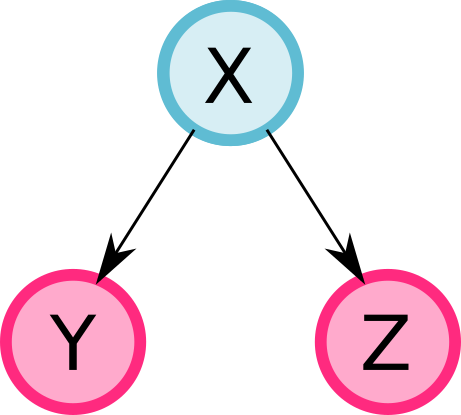
\includegraphics[scale=0.4]{Figures/ex1.png}
\end{figure}
\begin{figure}[h]
	\centering
	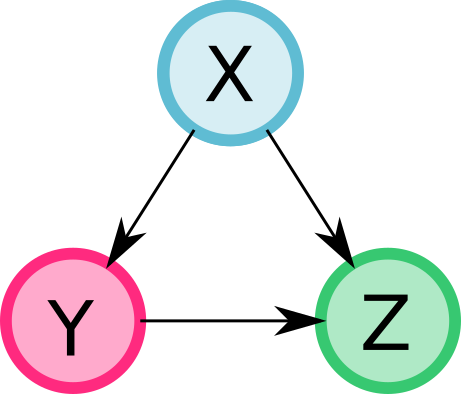
\includegraphics[scale=0.4]{Figures/ex2.png}
\end{figure}

Nullam semper quam at ante convallis posuere. Ut faucibus tellus ac massa luctus consectetur. Nulla pellentesque tortor et aliquam vehicula. Maecenas imperdiet euismod enim ut pharetra. Suspendisse pulvinar sapien vitae placerat pellentesque. Nulla facilisi. Aenean vitae nunc venenatis, vehicula neque in, congue ligula.

Pellentesque quis neque fringilla, varius ligula quis, malesuada dolor. Aenean malesuada urna porta, condimentum nisl sed, scelerisque nisi. Suspendisse ac orci quis massa porta dignissim. Morbi sollicitudin, felis eget tristique laoreet, ante lacus pretium lacus, nec ornare sem lorem a velit. Pellentesque eu erat congue, ullamcorper ante ut, tristique turpis. Nam sodales mi sed nisl tincidunt vestibulum. Interdum et malesuada fames ac ante ipsum primis in faucibus.

\begin{figure}[h]
	\centering
	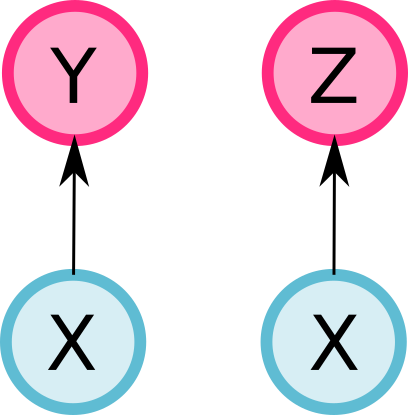
\includegraphics[scale=0.4]{Figures/ex1input.png}
\end{figure}
\begin{figure}[h]
	\centering
	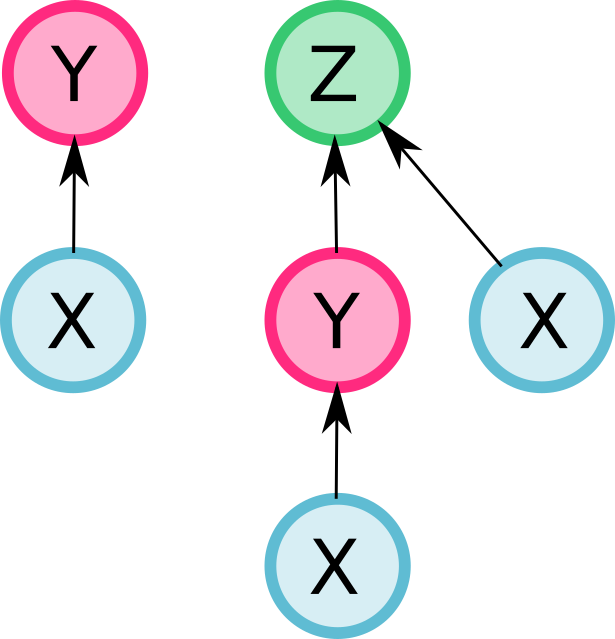
\includegraphics[scale=0.4]{Figures/ex2input.png}
\end{figure}

%------------------------------------------------

\section{\textit{Coarsest Refinement Partitioning }Algorithm}

To identify the correct distribution of fibers over the network it is necessary to define an efficient procedure to split the nodes into different disjoint partitions, from which all nodes inside the same partition must receive equivalent information from all other partitions. To do that, we treat our problem as the same as finding the coarsest relational refinement partitioning of a set of elements that have a binary relation between them. Since a network is completely defined by a set of node elements and a set of edges that comprehend all the binary relations, this approach can be used. Therefore, in this section, I detail the optimal algorithm used to find this coarsest partitioning in the context of graph fibrations and show the relatively simple implementation of this method.

The algorithm used in this project is a slightly modified version of the algorithm presented by Paige and Tarjan \cite{Tarjan1987}, \ having a runtime complexity of $\mathcal{O}(M\log N)$, where $M$ and $N$ are, respectively, the number of edges and nodes in the network, being almost linear with the size of the network. It is important to note that this algorithm has the same runtime order than the algorithm from Cardon and Crushemore \cite{Cardon1982}, in which the algorithm of minimal fibration from \cite{fibration2019} is based. However, the algorithm presented by Paige and Tarjan has a simpler implementation and smaller prefactors, exhibiting a better approach to our problem. Even though the algorithm has wider general applications, here I give the details of the algorithm implementation to the application for a network, so that I introduce the necessary definitions within this context.

\subsection{Algorithm description}

A network $G(V, E)$ is completely defined by the sets of the nodes elements $V$ and the set of the edges $E$. The network has $N = |V|$ nodes that can have connections with one another defined by the set $E$, which contains $M = |E|$ ordered pair of nodes, denoting the directed links between the network nodes. Considering the network, we can define a graph partition $\bar{P}$ over $V$ as a set of pairwise disjoints subsets of $V$ whose union is all $V$, that is
\begin{equation}
	\bar{P} = \bigcup_{i} P_i
\end{equation}
where $P_i$ are the elements of the partition $\bar{P}$, called blocks. Considering this, if we take an additional graph partition $\bar{Q}$ that has the property that all of its blocks are contained in a block of $\bar{P}$, we say that $\bar{Q}$ is a refinement partition of $\bar{P}$.

Moreover, for a block $B \in \bar{P}$, we say that the block $B$ is stable with respect with a set $S$ if either all elements of $B$ connects with an element of $S$ or none element of $B$ points to any element of $S$. The stability partition concept is central to the problem of relational coarsest refinement partitioning and can be easily extended to graph problems, where the coarsest graph partition problem is that of finding, for a given set of connections $E$ and an initial partition $\bar{P}$ over $V$, the coarsest stable refinement of $\bar{P}$, i. e., the minimal number of disjoint blocks subsets of $V$ that forms a stable refinement of $\bar{P}$. 

Considering the stability of partitions, for a proper identification of the network fibers as defined in the above section we ought to construct a stable graph partition that is equivalent to the coarsest refinement of the network (minimal number of blocks) with respect to the information processing of each node. For that goal, we need to extend the concept of stability over partitions for the case that accounts for the information processed by each block of the partition. Therefore, to identify the group of nodes with isomorphic input-tree, we require that the partition should be not only stable but \textbf{input-tree stable}. That means that for a subset $S \subseteq$ $V$, a graph partition $\bar{P}$ over the network $G(V, E)$ is input-tree stable with respect to $S$ if for all the block $B \in \bar{P}$, the following equality is satisfied for all the elements $x$, $y \in B$:
\begin{equation}
	| E^{-1}(\{x\}) \cap S | = | E^{-1}(\{y\}) \cap S |
\end{equation}
where $E(\{x\})$ and $E^{-1}(\{x\})$ represents, respectively, the set of nodes that directly receives information from $x$, and the set of nodes that sends information, via a direct link, to $x$. 

This way, we can benefit from the stability properties \cite{Tarjan1987} to construct a refinement algorithm step that can achieve, through a finite number of steps, a input-tree stable partition from an initial unstable partitioning of the network. This way, given a subset $S \subseteq V$, the refinement step has the effect to refine the current partition, input-tree unstable with respect to $S$, by replacing it for a new partition, now input-tree stable for $S$. With that objective, we define a split function \textit{I-split($S$, $\bar{P}$)} that receive as input the current partition and a set $S$ and returns as output a new input-tree stable partition with respect to $S$. Favorably, that function benefits from two major properties of stability (and input-tree stability): the stability inheritance by refinement and by union of sets. By reason of this refinement inheritance, a given set $S$ can be used only once by the function \textit{I-split}, guaranting that the partition, after all other refinement steps, will maintain as stable with respect to $S$. Moreover, since stability is inherited under union of sets $S$, after sets are used in \textit{I-split}, their union cannot be used for the function. Considering all these properties, the essence of the refinement algorithm can be stated as

\begin{quotation}
	\textbf{Refinement Algorithm}: Find a set $S$ in which the current partition $\bar{P}$ is input-tree unstable. Replace $\bar{P}$ by the output of \textit{I-split($S$,$\bar{P}$)}. Guarantees that the set $S$ or unions of used sets never be used again.
\end{quotation}

Since the finest partitioning possible is the one in which every node is itself a block, the refinement step may be proceeded at most $N-1$ times, guaranting that the algorithm terminates with the correct answer, since stability is inherited by the refinement process. However, to guarantees that the algorithm has a optimal runtime we have to find a efficient way to select the appropriate sets to the refinement step, without choosing repeated ones. Fortunately, this can be easily done for the construction of a input-tree stable partition.

Given a set $S$ of nodes from the network $G(V, E)$ and a given input-tree unstable graph partition $\bar{P}$, the blocks $B \in \bar{P}$ that are input-tree unstable with respect to $S$ can be splitted into several blocks $B_j$ that will be stable input-tree with respect to $S$. Then, each splitted block will have the property defined by
\begin{equation}
	B_j = \{ x \in B : | E^{-1}(\{x\}) \cap S | = j \}
\end{equation}
where the number of splitted block must be larger than one to a proper splitting process take place. Then, for each unstable block $B \in \bar{P}$ all the splitted block, except the largest one, can be put at the back of a queue to be used ahead in the algorithm as a refinement set. This ensures that none repeated sets or union of repeated sets can be used during the algorithm exeecution.

Finally, having said all that, the complete algorithm to find the correct network fibers of a network $G(V, E)$ consists in initializing a graph partition $\bar{P}$ over all nodes from $V$ except the nodes that do not receive information from any other node, in which each one of these will be defined as isolated fibers already in the beginning of the algorithm. The partition $\bar{P}$ is defined as one block containing all the other nodes in the network. The algorithm maintains a queue $L$ of possible refinement sets, initially containing the single block of $\bar{Q}$ and all the isolated blocks defined at the beginning. Then, we proceed as
\begin{quotation}
	\textbf{Coarsest Refinement Algorithm}: Remove from $L$ its first set $S$. Replace $Q$ by the \textit{I-split($S$, $Q$)}. Whenever a block $B \in Q$ splits into two or more nonempty blocks, add all but the largest to the back of $L$.
\end{quotation}
And this process is repeated until the queue $L$ is empty. At this point, the resulted partition $\bar{P}$ represents the coarsest input-tree stable partitioning of the network $G(V, E)$, where each block represents a network fiber with all its nodes having isomorphic input-trees.

% faltou o preprocessing.

\subsection{Data preparation and algorithm implementation}

We apply the above algorithm in the genetic regulatory network of the \textit{Escherichia Coli} bacteria. We obtain the genetic E. Coli network through its transcriptional regulatory interactions data, where each gene is regulated by a transcription factor protein. Since a transcription factor production in the cell is regulated by a gene, we can define a directed connection between two genes if a gene regulates the production of a transcriptional factor, which it regulates another gene. Since a transcription factor can be either an activator(positive) or repressor(negative), or even behaves as both(dual), the links between genes can carry different types of messages. Because of that, it is important that the partitioning algorithm accounts the type of message to construct appropriate input-trees for the network fibers partition. Therefore, for a proper application of the algorithm on the \textit{Escherichia Coli} genetic network, we label each node uniquely, either as number or string names, and also each link with the type of connection between genes.

Considering this context, we explain now how the algorithm should proper be implemented to have an optimal perfomance concerning its runtime complexity. After discussing the data structures necessary to deal correctly with data, we design an algorithm recipe to show all the main steps of the process explained above. Also, anyone can acess our own personal implementation for genetic regulatory networks in the link \url{https://github.com/higorsmonteiro/fiberblocks} on github platform.

Given a directed network $G(V, E)$ to be partitioned in fibers, it is very important for the correctness of the algorithm that the nodes that do not receive any information, that is, the nodes that do not have any inward connections, be preprocessing as isolated blocks. This means that the initial graph partition $P$ is divided in two different partition $P'$ e $P''$, the first one contained all the single-node blocks containing the solitaire nodes $v$ in which $| E^{-1}(\{v\}) | = 0$, and the second one containing initialing a single block containing all the other nodes $w$ in which $| E^{-1}(\{w\}) | \geq 1$. The importance of this preprocessing is to guarantee that solitaire nodes do not be put on the same fibers during the refinement steps. Even though the blocks of $P'$ are used as refinement sets, $P'$ is not used by the algorithm. Thus, the final partition is the union of $P'$ and the result of the refinement partitioning of $P''$.

After the above preprocessing we define the data structures for the partition $Q$ for its blocks $B$. A partition is a doubly linked list of blocks, which allows that deletion of blocks be made in constante time $O(1)$ as long we have the block memory address during the procedure. A block is just a structure containing indexing data along with a doubly linked list containg all the nodes that belongs to it. Together with a queue of blocks $L$, these constructions are the main data structures necessary for an efficient implementation of the refinement partitioning algorithm. At the beginning of the algorithm, we enqueue all the blocks of $P'$ e $P''$ to $L$. Then, we start the algorithm initializing a partition $Q = P''$ and by removing the top element set $S$ of $L$, then we apply the \textit{I-split($S$, $Q$)} to identify the input-tree unstable blocks of $Q$ and split them into input-tree stable blocks with respect to  $S$. This way, all the splitted blocks are push to the end of $L$, with exception the largest resulted blocks for each splitted block. As we have mentioned, the algorithm terminates when there is no more sets in $L$. Even though this is the whole algorithm, the implementation of the \textit{I-split} function might not be so straightforward, since a given block $B$ can be splitted into an arbitrary number of blocks. In respect to that below we propose the following implementation construction to the splitting function:

\begin{algorithm}[h]
	\SetAlgoLined
	\SetKwInOut{Input}{Input}
    \SetKwInOut{Output}{Output}
	\Input{A set $S$ and a partition $\bar{Q}$}
    \Output{Input tree stable partition $\bar{Q}$ with respect to $S$}
	%\KwResult{}
	Initialize $\bar{U}$ as an empty partition\;
	\For{$\forall B \in \bar{Q}$}
	{
		\If{$\exists \ \{ w_i, w_j \} \subseteq B : | E^{-1}(\{w_i\})\cap S | \neq | E^{-1}(\{w_j\})\cap S |$}
		{
			\textit{push} $B$ to $\bar{U}$\;
			Initialize $\bar{T}$ as an empty partition\;
			\For{$\forall w_i \in B$}
			{
				\eIf{$\exists \ X \in \bar{T} : | E^{-1}(\{w_i\})\cap S | = X(E)$ }
				{
					insert $w_i$ in $X$\;
					
				}
				{
					create a new block $X$\;
					insert $w_i$ in $X$\;
					$X(E) \leftarrow | E^{-1}(\{w_i\})\cap S |$\;
					push block $X$ to $\bar{T}$ 
				}
			}
		}
		\textit{enqueue} all blocks $X \in \bar{T}$ in $L$, except the largest one\;
		\textit{push} all blocks $X \in \bar{T}$ to $\bar{Q}$\;
	}
	\textit{delete} all blocks $B \in \bar{U}$ in $\bar{Q}$
	\caption{\textit{I-split} $(S,\bar{Q}, L)$}
\end{algorithm}

In the algorithm recipe above, our \textit{I-split} function receives a set $S$ and the partition $\bar{Q}$ as input and returns a input-tree stable $\bar{Q}$ with respect to $S$ as output. Besides its list of nodes, a block $X$ has another attribute acessed as $X(E)$, which receives, during the splitting process, the number of inward links coming from the current refinement set $S$. This way, a node $w$ belonging to the block to be splitted can be put in the block $X \in \bar{T}$ that has the same attribute value, like stated in the conditional expression at line $7$ of the algorithm above.

Finally, considering all the discussion above, we can explicit the complete algorithm in just a few steps.

\begin{algorithm}[h]
	\SetAlgoLined
	\SetKwInOut{Input}{Input}
	\Input{A network $G(V, E)$}
	%\KwResult{}
	Initialize $S$ as an empty set\;
	Initialize $L$ as an empty queue\;
	Initialize $\bar{P}$, $\bar{P'}$, $\bar{P''}$, $\bar{Q}$ as empty partitions\;
	$B' = \{ \{ w \} \in V : |E^{-1}(\{w\})|=0 \}$\;
	$B'' = \{ v \in V : |E^{-1}(\{v\})| \geq 1 \}$\;
	\textit{push} all $B'$ to $\bar{P'}$\;
	\textit{push} $B''$ to $\bar{P''}$\;
	\textit{enqueue} $B'' \in \bar{P''}$ to $L$\;
	\textit{enqueue} all blocks $B' \in \bar{P'}$ to $L$\;
	$\bar{Q} \leftarrow \bar{P''}$\;
	\While{$|L| \neq 0$}
	{
		$S \leftarrow \text{\textit{dequeue}}(L)$\;
		$\bar{Q} \leftarrow \text{\textit{I-input}}(S, \bar{Q}, L)$
	}
	\caption{Coarsest Refinement Graph Partitioning}
\end{algorithm}

A concrete implementation of the algorithm in a programming language is presented at the link \url{https://github.com/higorsmonteiro/fiberblocks} together with \textit{E. Coli} prepared data and another examples. Further information about the application of the codes in other genetic regulatory network data can be found at the same link given.

%------------------------------------------------

\section*{Results}

Using the algorithm above, we applied it to a set of networks examples before its proper application on the \textit{Escherechia Coli} genetic regulatory network data. The reason for that is merely to show that the not just the algorithmic approach chosen is consistent but the written code per si is correctly implementated. For each network, we have a adjacency list containing all the directed connections between the nodes and for each connection we have a string defining the type of regulation of a specific link, where here, considering the genetic regulation context, the types can be positive, negative or dual. The first three examples are all small networks, containing at most $48$ nodes, and so all can be used to test the correctness of the algorithm applied. For that three examples we show the network drawing and their fibers distribution identified as the result of the algorithm.

The first example is showed at the figure \ref{fig:result1}. This network is disconnected, containing two main weakly connected components, and contains only positive regulation between the interactions between the genes, showing the simpler case where the connections between nodes in a network are all of the same type. In this case, we find five non-trivial fibers, that is, fibers with size larger than one.

\begin{figure}[h]
	\centering
	\subfloat[]{{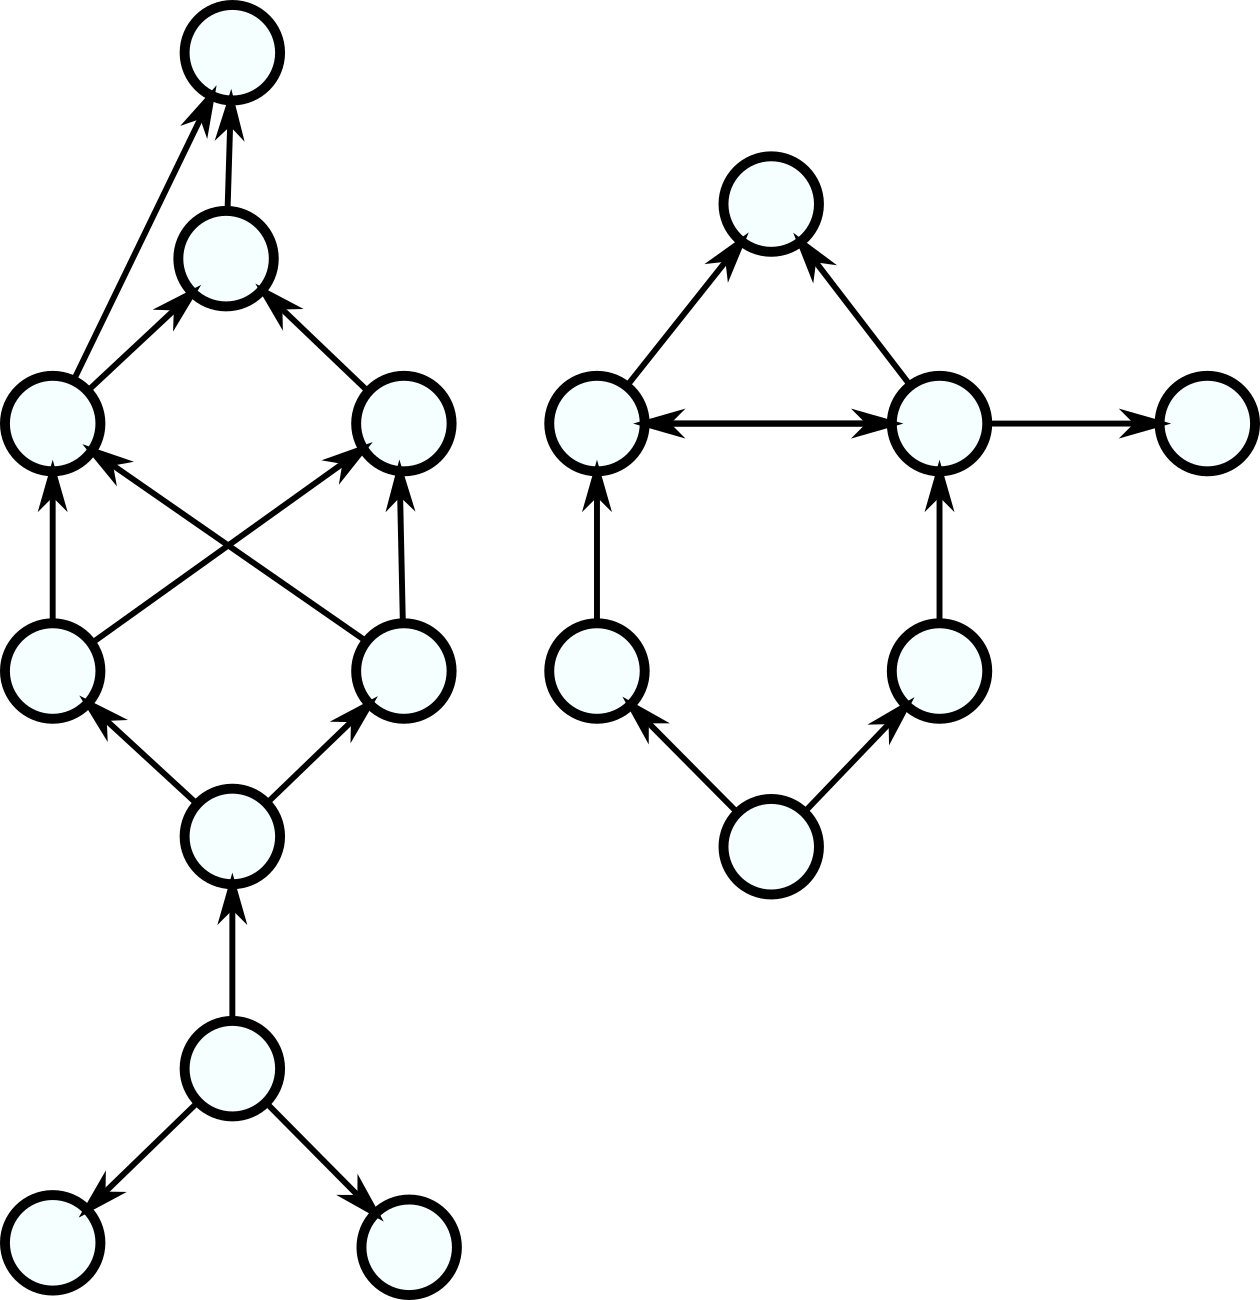
\includegraphics[scale=0.3]{Figures/result1.png}}}
	\qquad
	\subfloat[]{{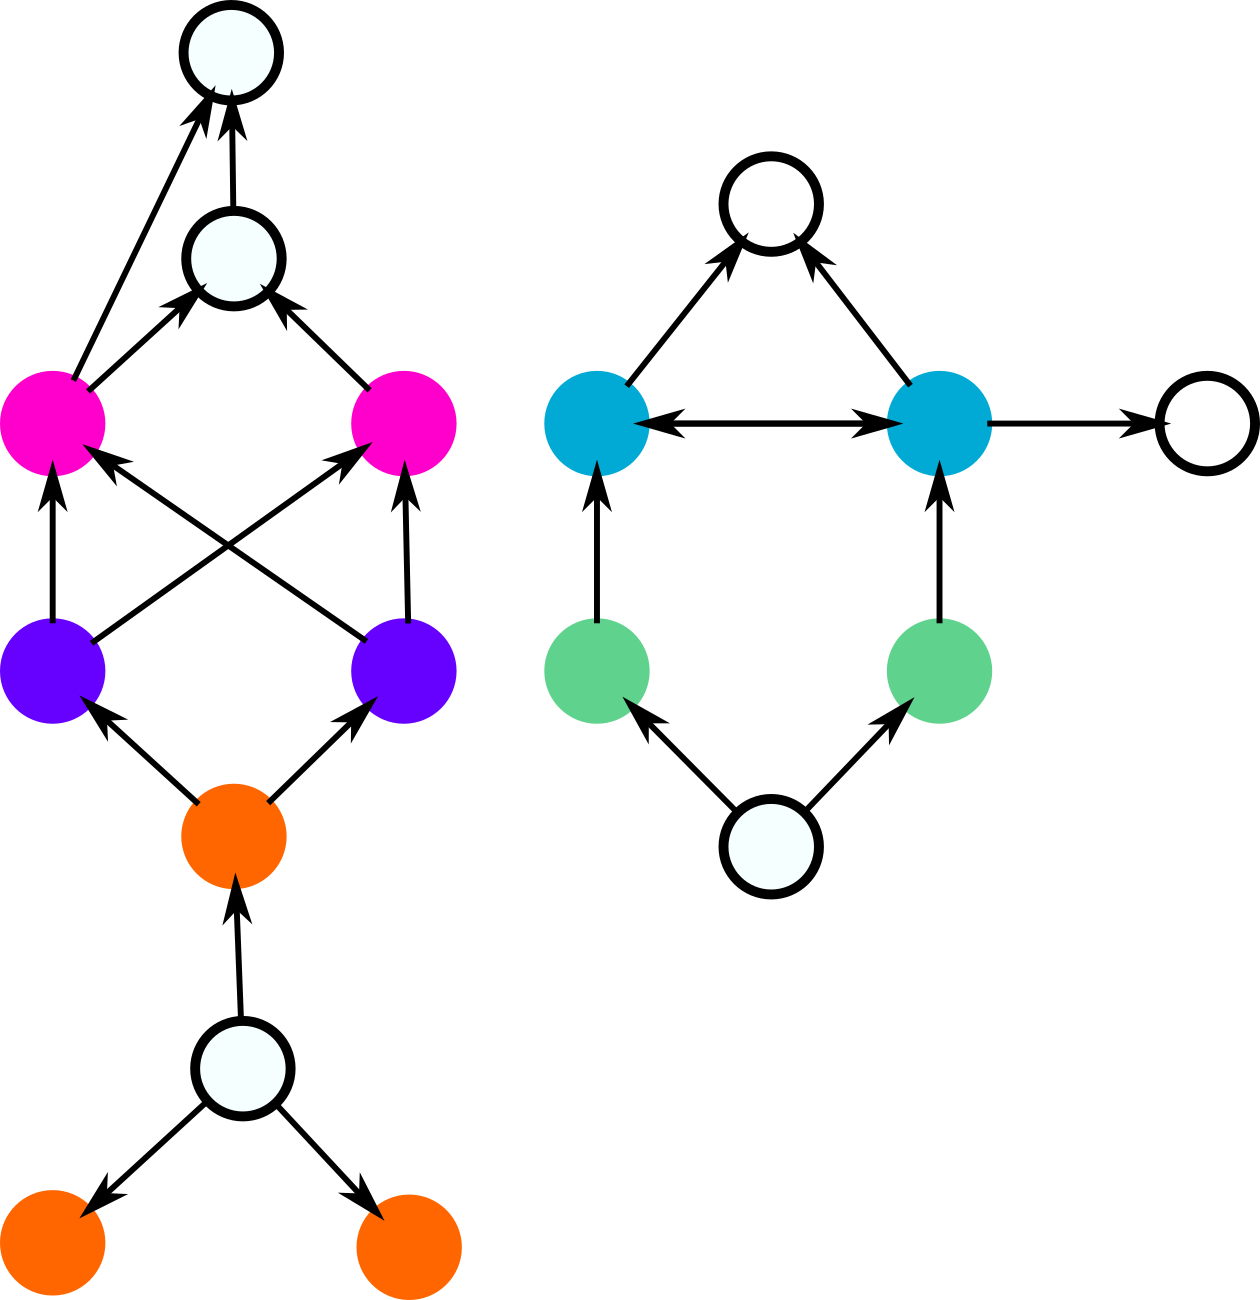
\includegraphics[scale=0.3]{Figures/result1-1.png}}}
	\caption{}
	\label{fig:result1}
\end{figure}

At the end of the algorithm, all the fibers identified are input-tree stable with respect to all fibers in the network, including the fiber itself. Then, labelling each fiber by an index or color we can then construct the fibration building blocks through the calculation of the fundamental class number $n$ and through the subclass number $l$. Again, a fibration building block is defined as the nodes inside the fiber as well as the $l$ external nodes that directly regulates at least one node of the current fiber. By that, we calculate the fundamental class number $n_k$ of the fiber $k$ by constructing the adjacency matrix $A_{ij}^{k}$ of its fibration building block and then calculating the largest eigenvalue of it. The value of $n$ quantifies the information loops of the fibration building blocks and can be either a integer or fractal golden ration.

Labelling the resulted fiber distribution, we obtain the following fibration classification for each fibratiion buuilding block of the network containing more than one node:

\begin{figure}[!ht]
    \centering
    \subfloat[]{{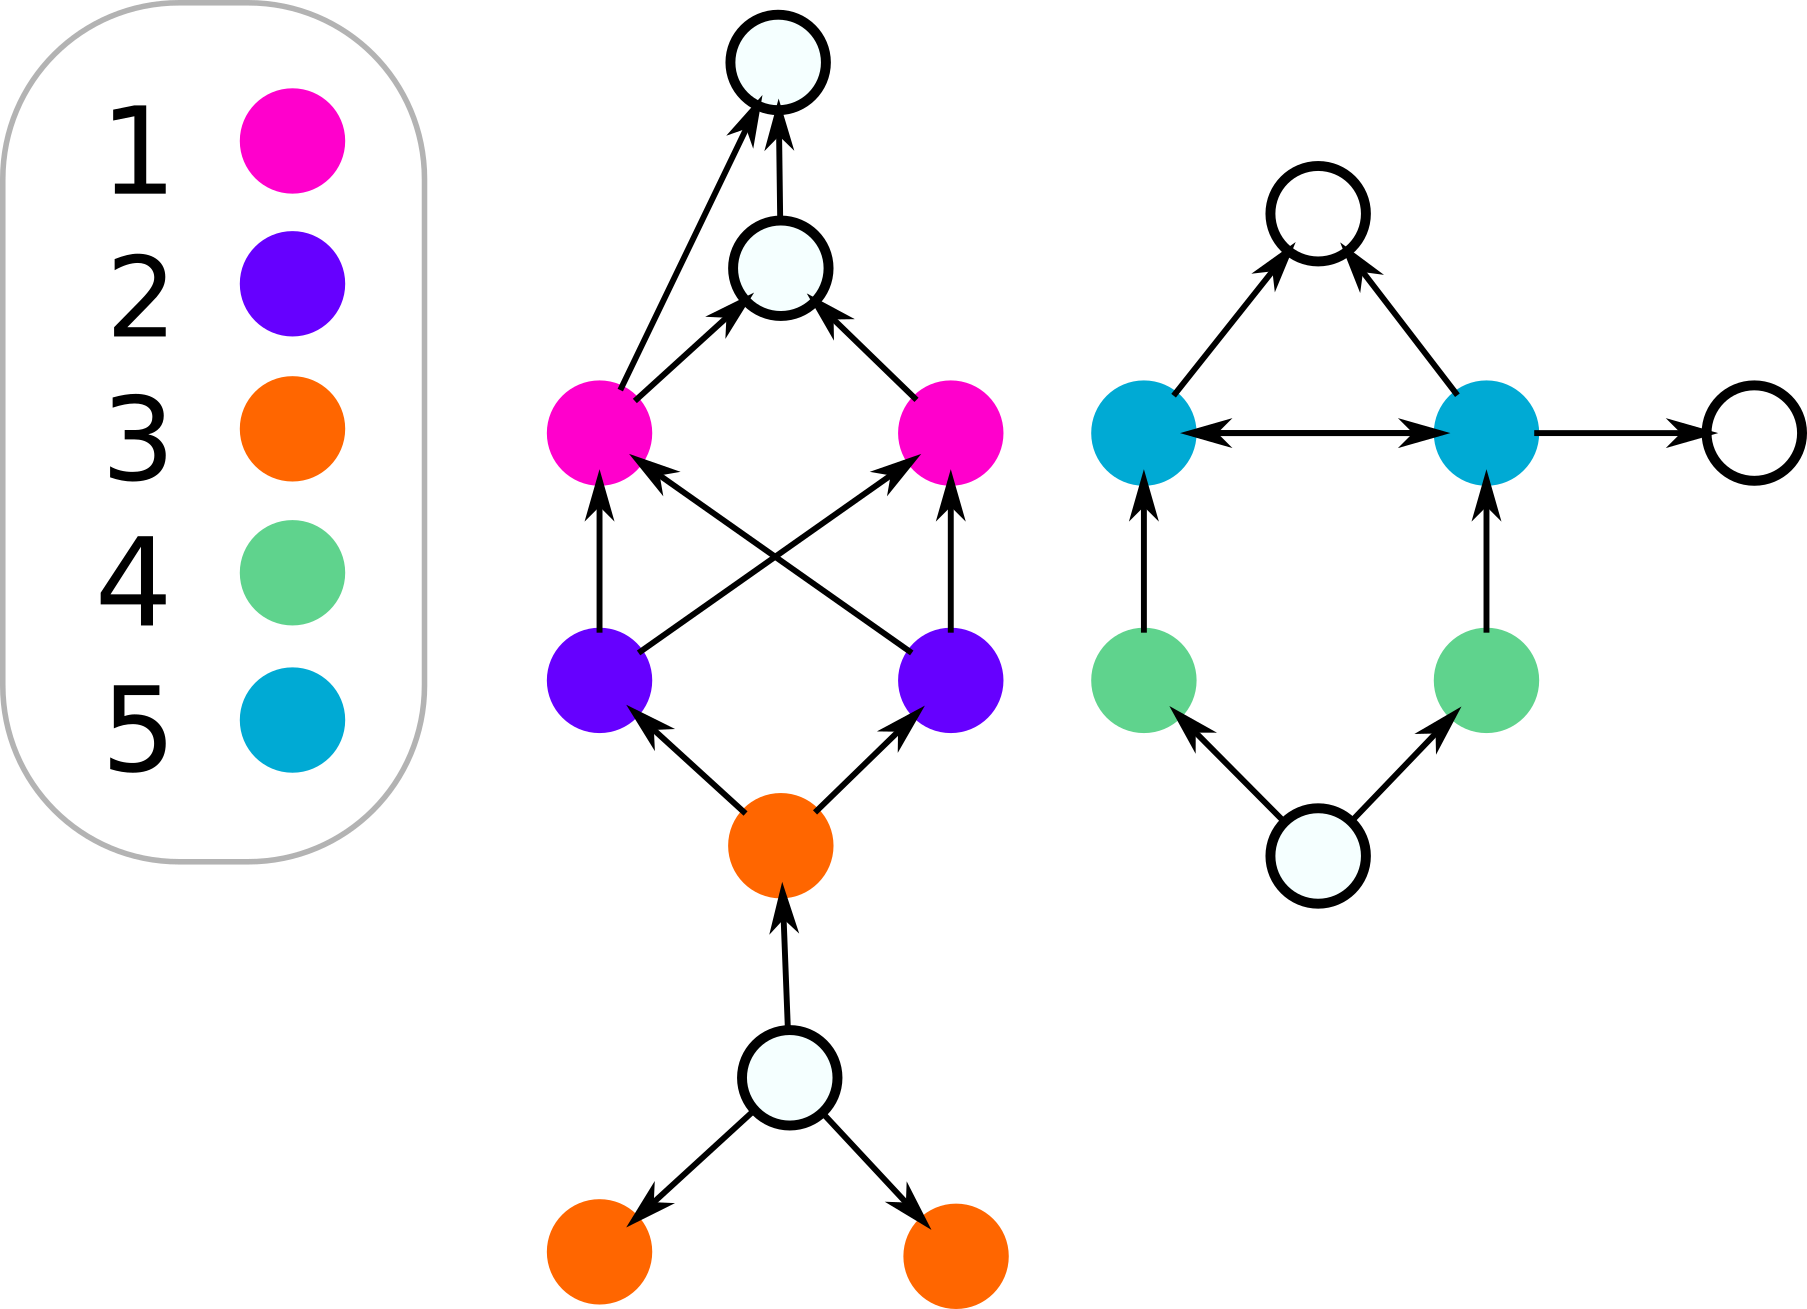
\includegraphics[scale=0.22]{Figures/result1-label.png}}}
    \qquad
    \begin{tabular}[b]{cc}\hline
      Table head & Table head \\ \hline
      Some values & Some values \\
      Some values & Some values \\
      Some values & Some values \\
      Some values & Some values \\
      Some values & Some values \\
      Some values & Some values \\ \hline
    \end{tabular}
    %\captionlistentry[table]{A table beside a figure}
    %\captionsetup{labelformat=andtable}
    %\caption{A table beside a figure}
\end{figure}

The second example exhibits a connected component containing $N = 21$ nodes, where all the three type of regulation are present. For this network we find the total of eleven fibers, where just six are fibers containing more than one node in it. As we can notice, for two arbitrary nodes be in the same fiber they must not just receive the same number of inward connections but the same number of each type of inward connections, this way receive the equivalent information from the rest of the network. We can see this for the example of the fibers $4$ e $5$, where even though both receives two links from the same central node, the fibers receives different types of information from that node, meaning that they are not the equivalent fibers.

\begin{figure}[H]
	\centering
	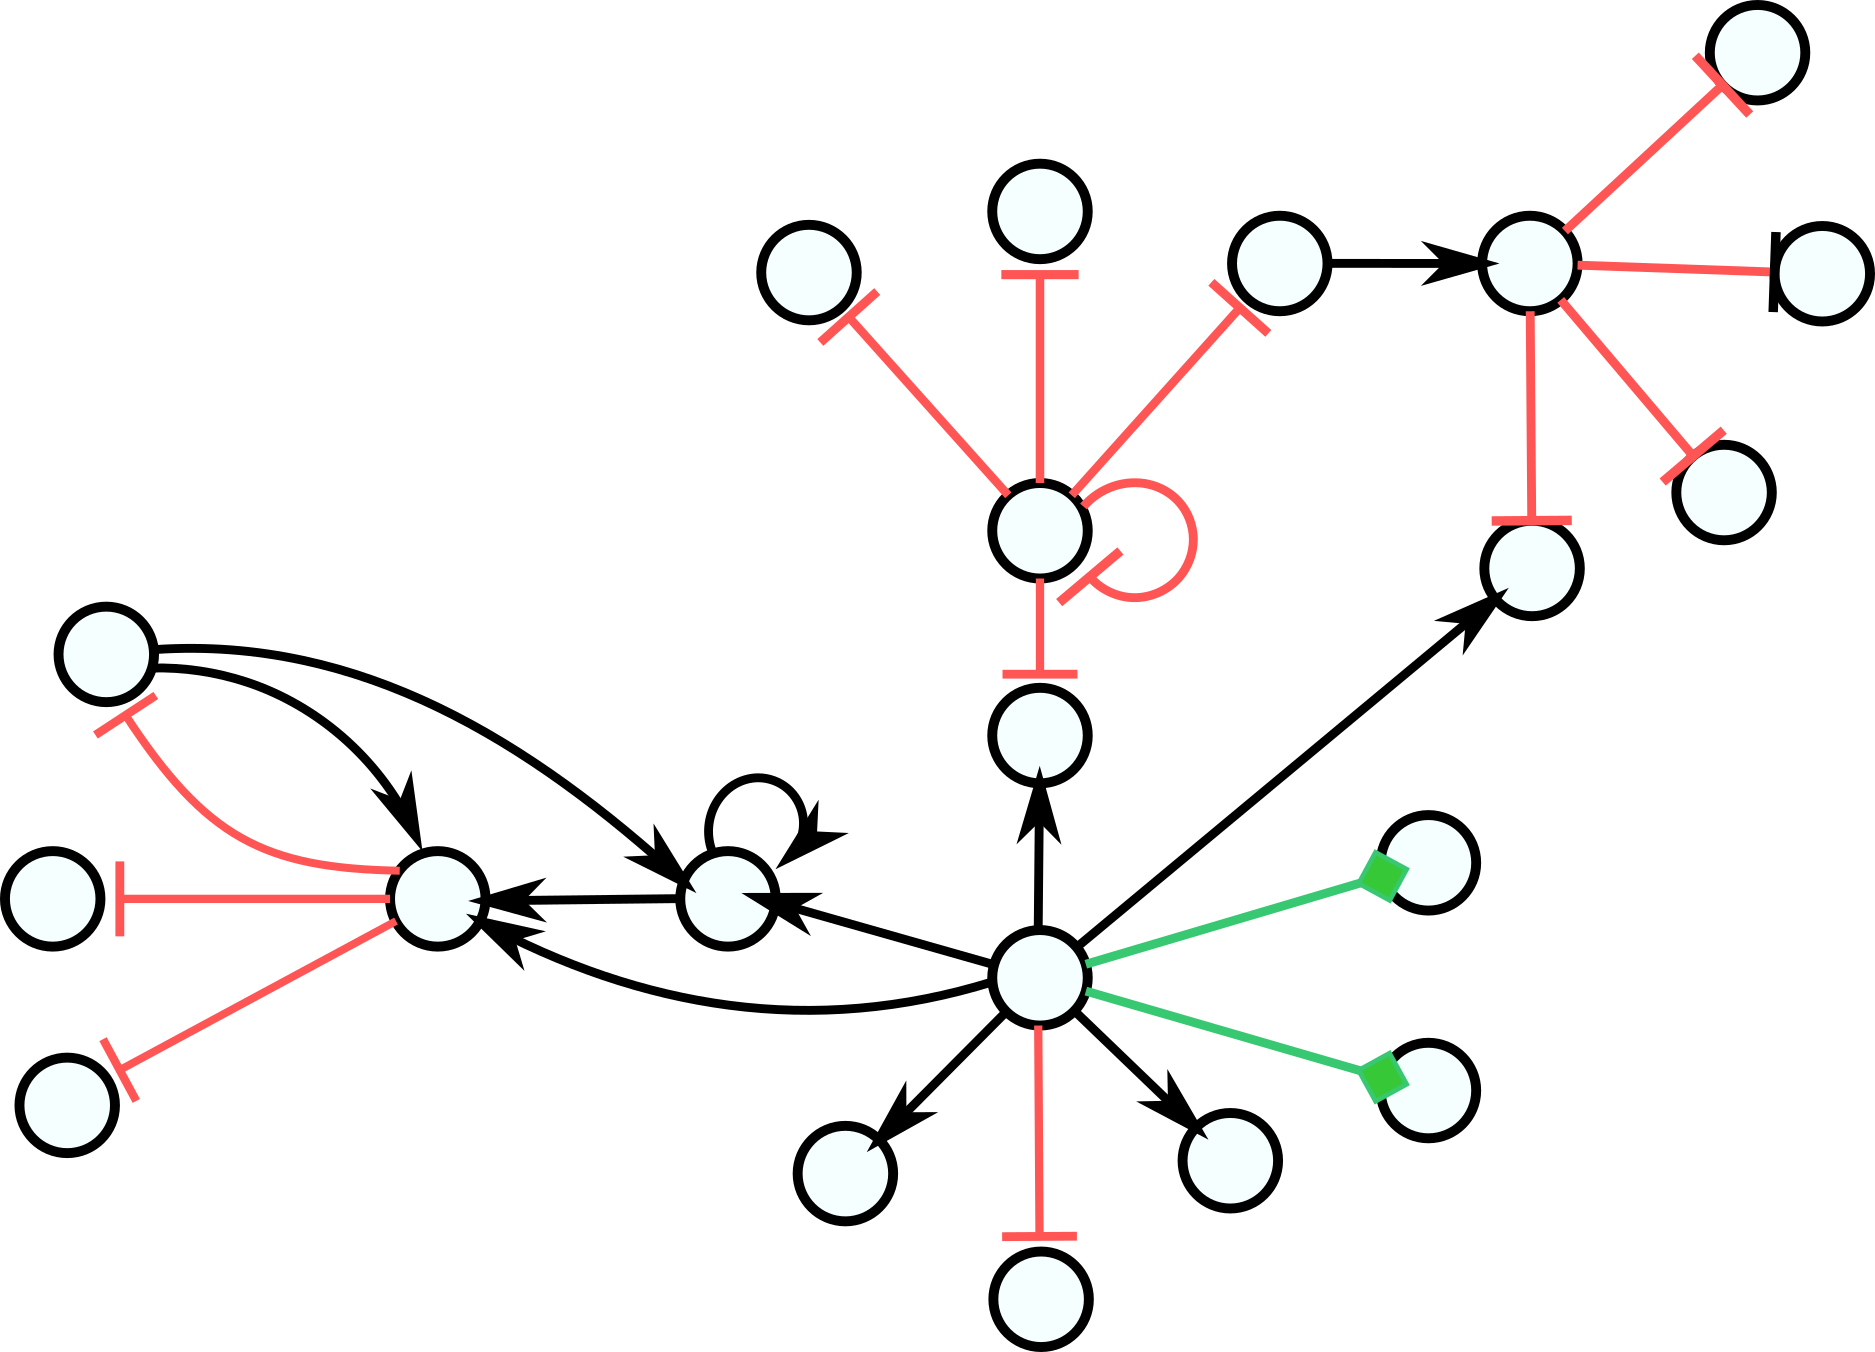
\includegraphics[scale=0.3]{Figures/result2.png}
\end{figure}
\begin{figure}[H]
	\centering
	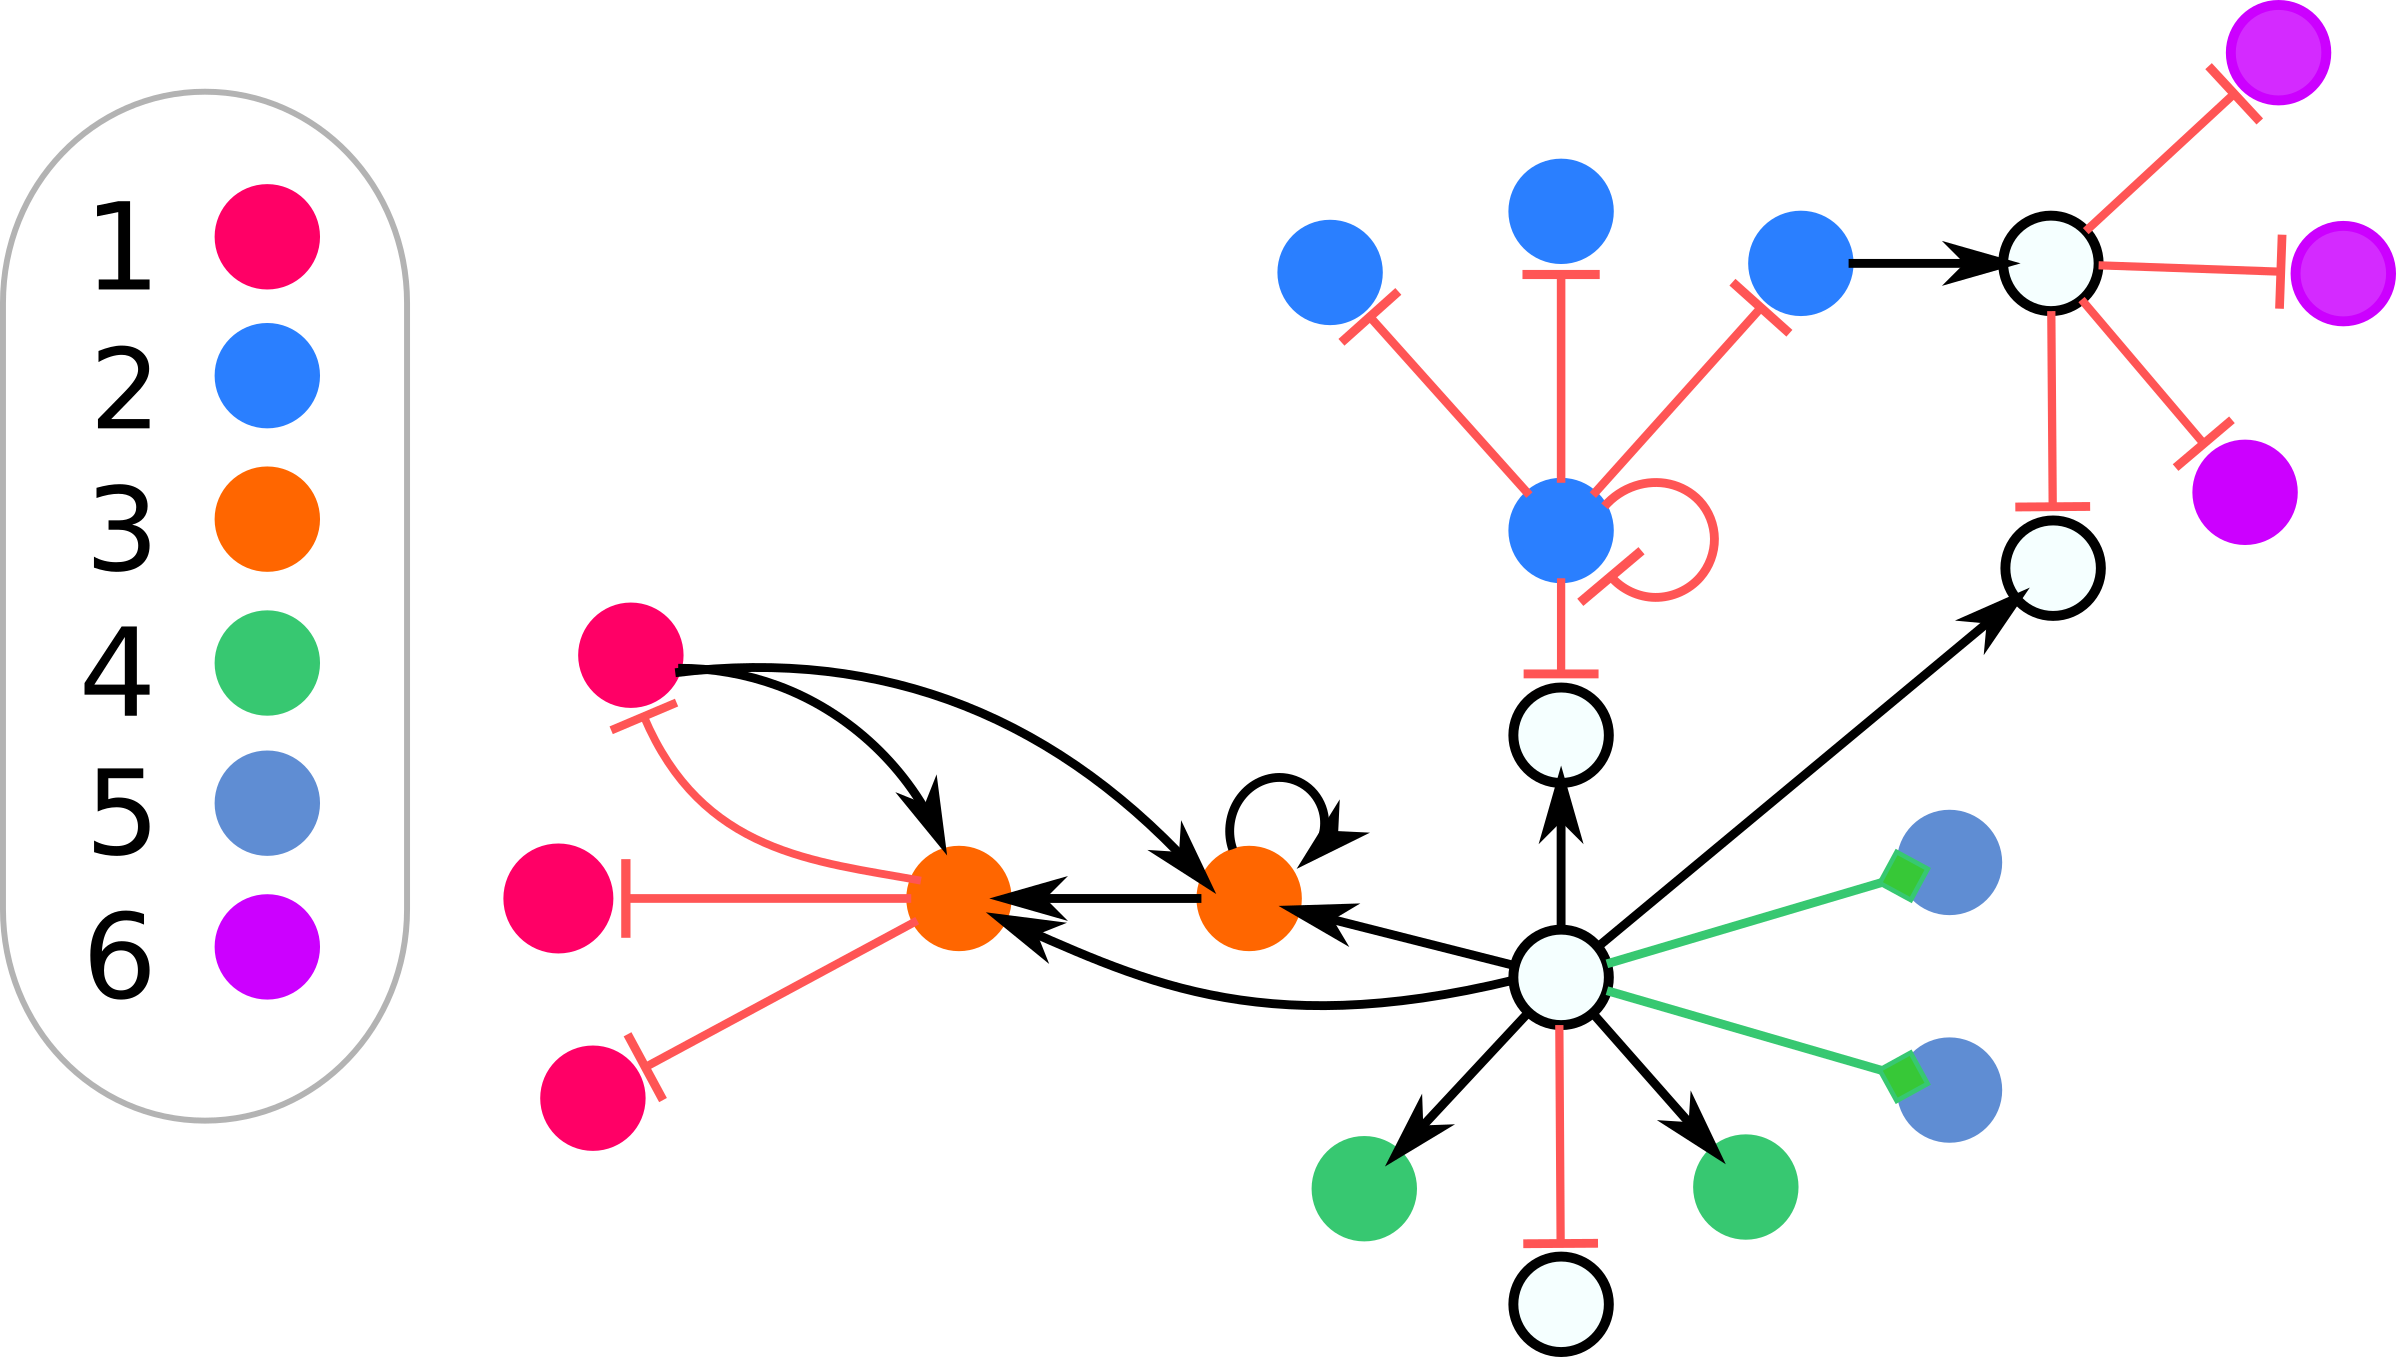
\includegraphics[scale=0.3]{Figures/result2-label.png}
\end{figure}

If we consider the fiber $3$, besides the inner autoregulation loop we have a loop information going outside the fiber and going back through an external regulator inside the fiber $1$. In cases like this the branching ratio of the fiber has a fractal value represented by a golden ratio $\phi_d$ resulted a loop information represented by a fibonacci sequence. This way, fiber $3$ can be classified by the values $| \phi_d, l = 2 \rangle$ where the fiber has two external regulator nodes. The fibration classification for the non-trivial fibers is showed in the table \ref{asdas}.

\begin{table}
\centering
\begin{tabular}[b]{cc}\hline
	Table head & Table head \\ \hline
	Some values & Some values \\
	Some values & Some values \\
	Some values & Some values \\
	Some values & Some values \\
	Some values & Some values \\
	Some values & Some values \\ \hline
  \end{tabular}
\end{table}

Before applying the algorithm for the whole network, we chose, for the finality of visualization and testing, to apply first the algorithm for a weakly connected component of the \textit{E. Coli} network. The same network is showed at the supplementary information from \cite{fibration2019}. The fiber distribution found is consistent with the one presented at \cite{fibration2019}, presenting the total of fifteen non-trivial fiber groups as shown in figure \ref{fig:result3-1}.

\begin{figure}[H]
	\centering
	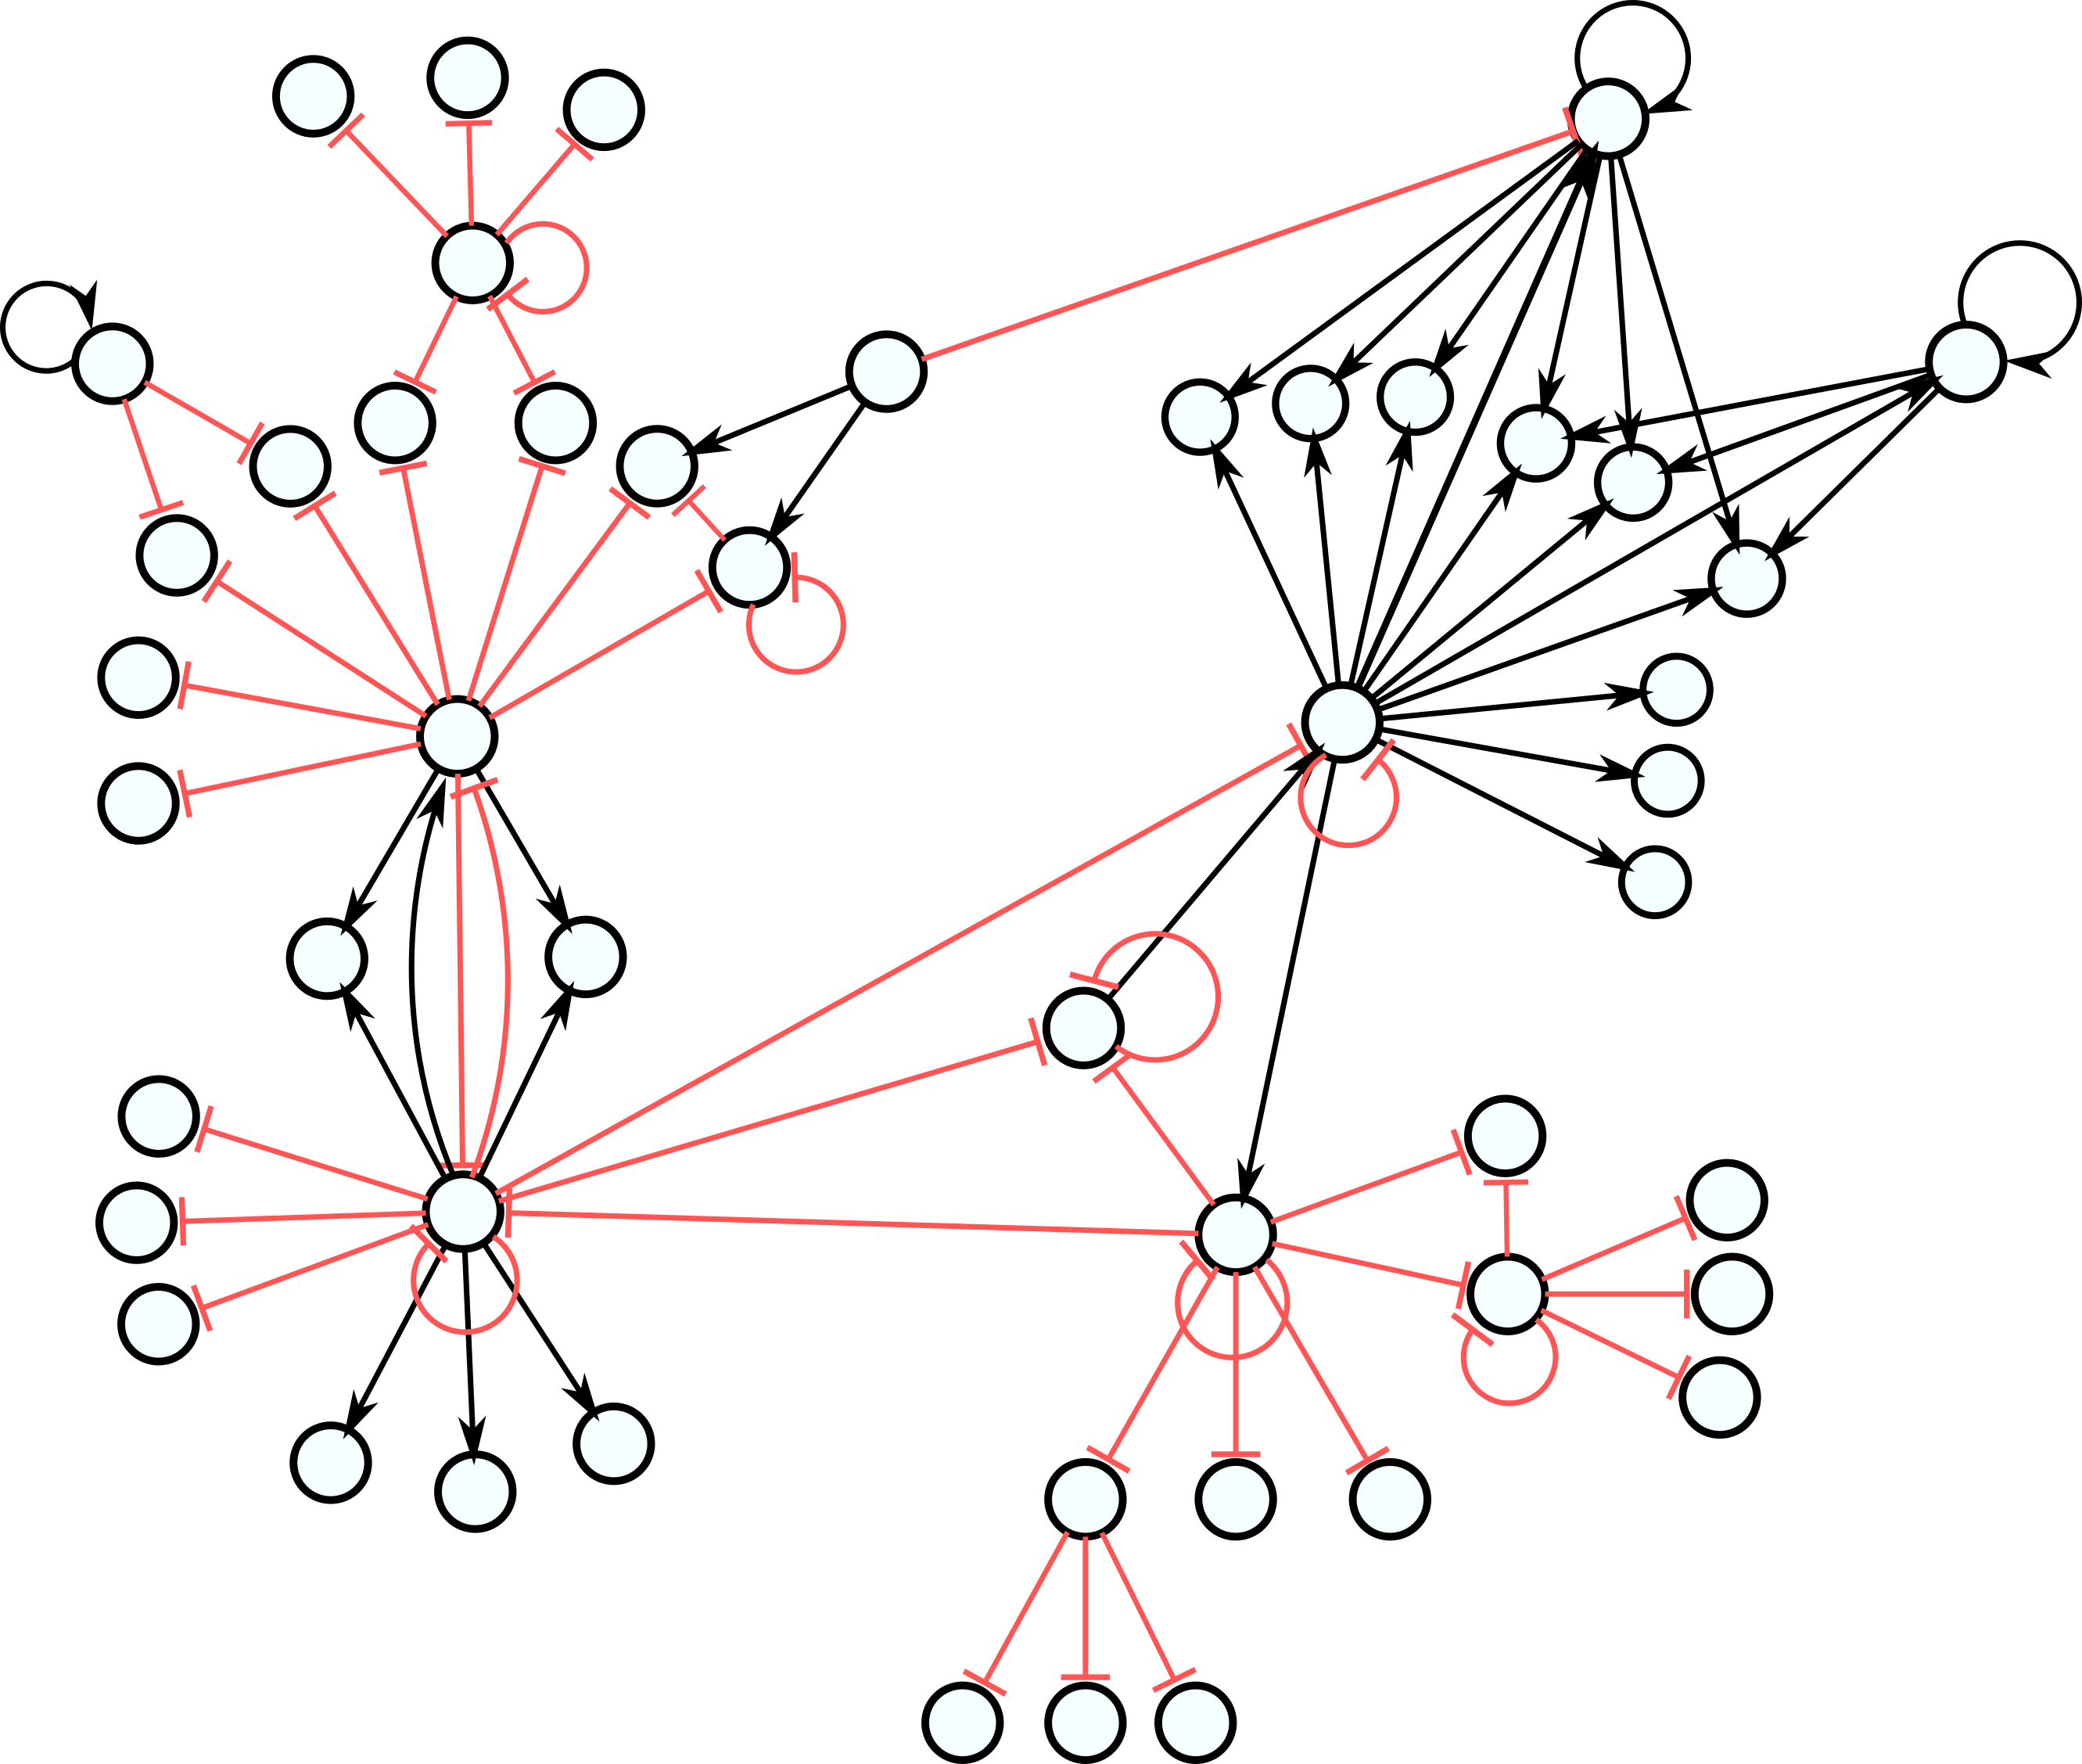
\includegraphics[scale=0.27]{Figures/result3.png}
	\caption{}
	\label{fig:result3}
\end{figure}
\begin{figure}[H]
	\centering
	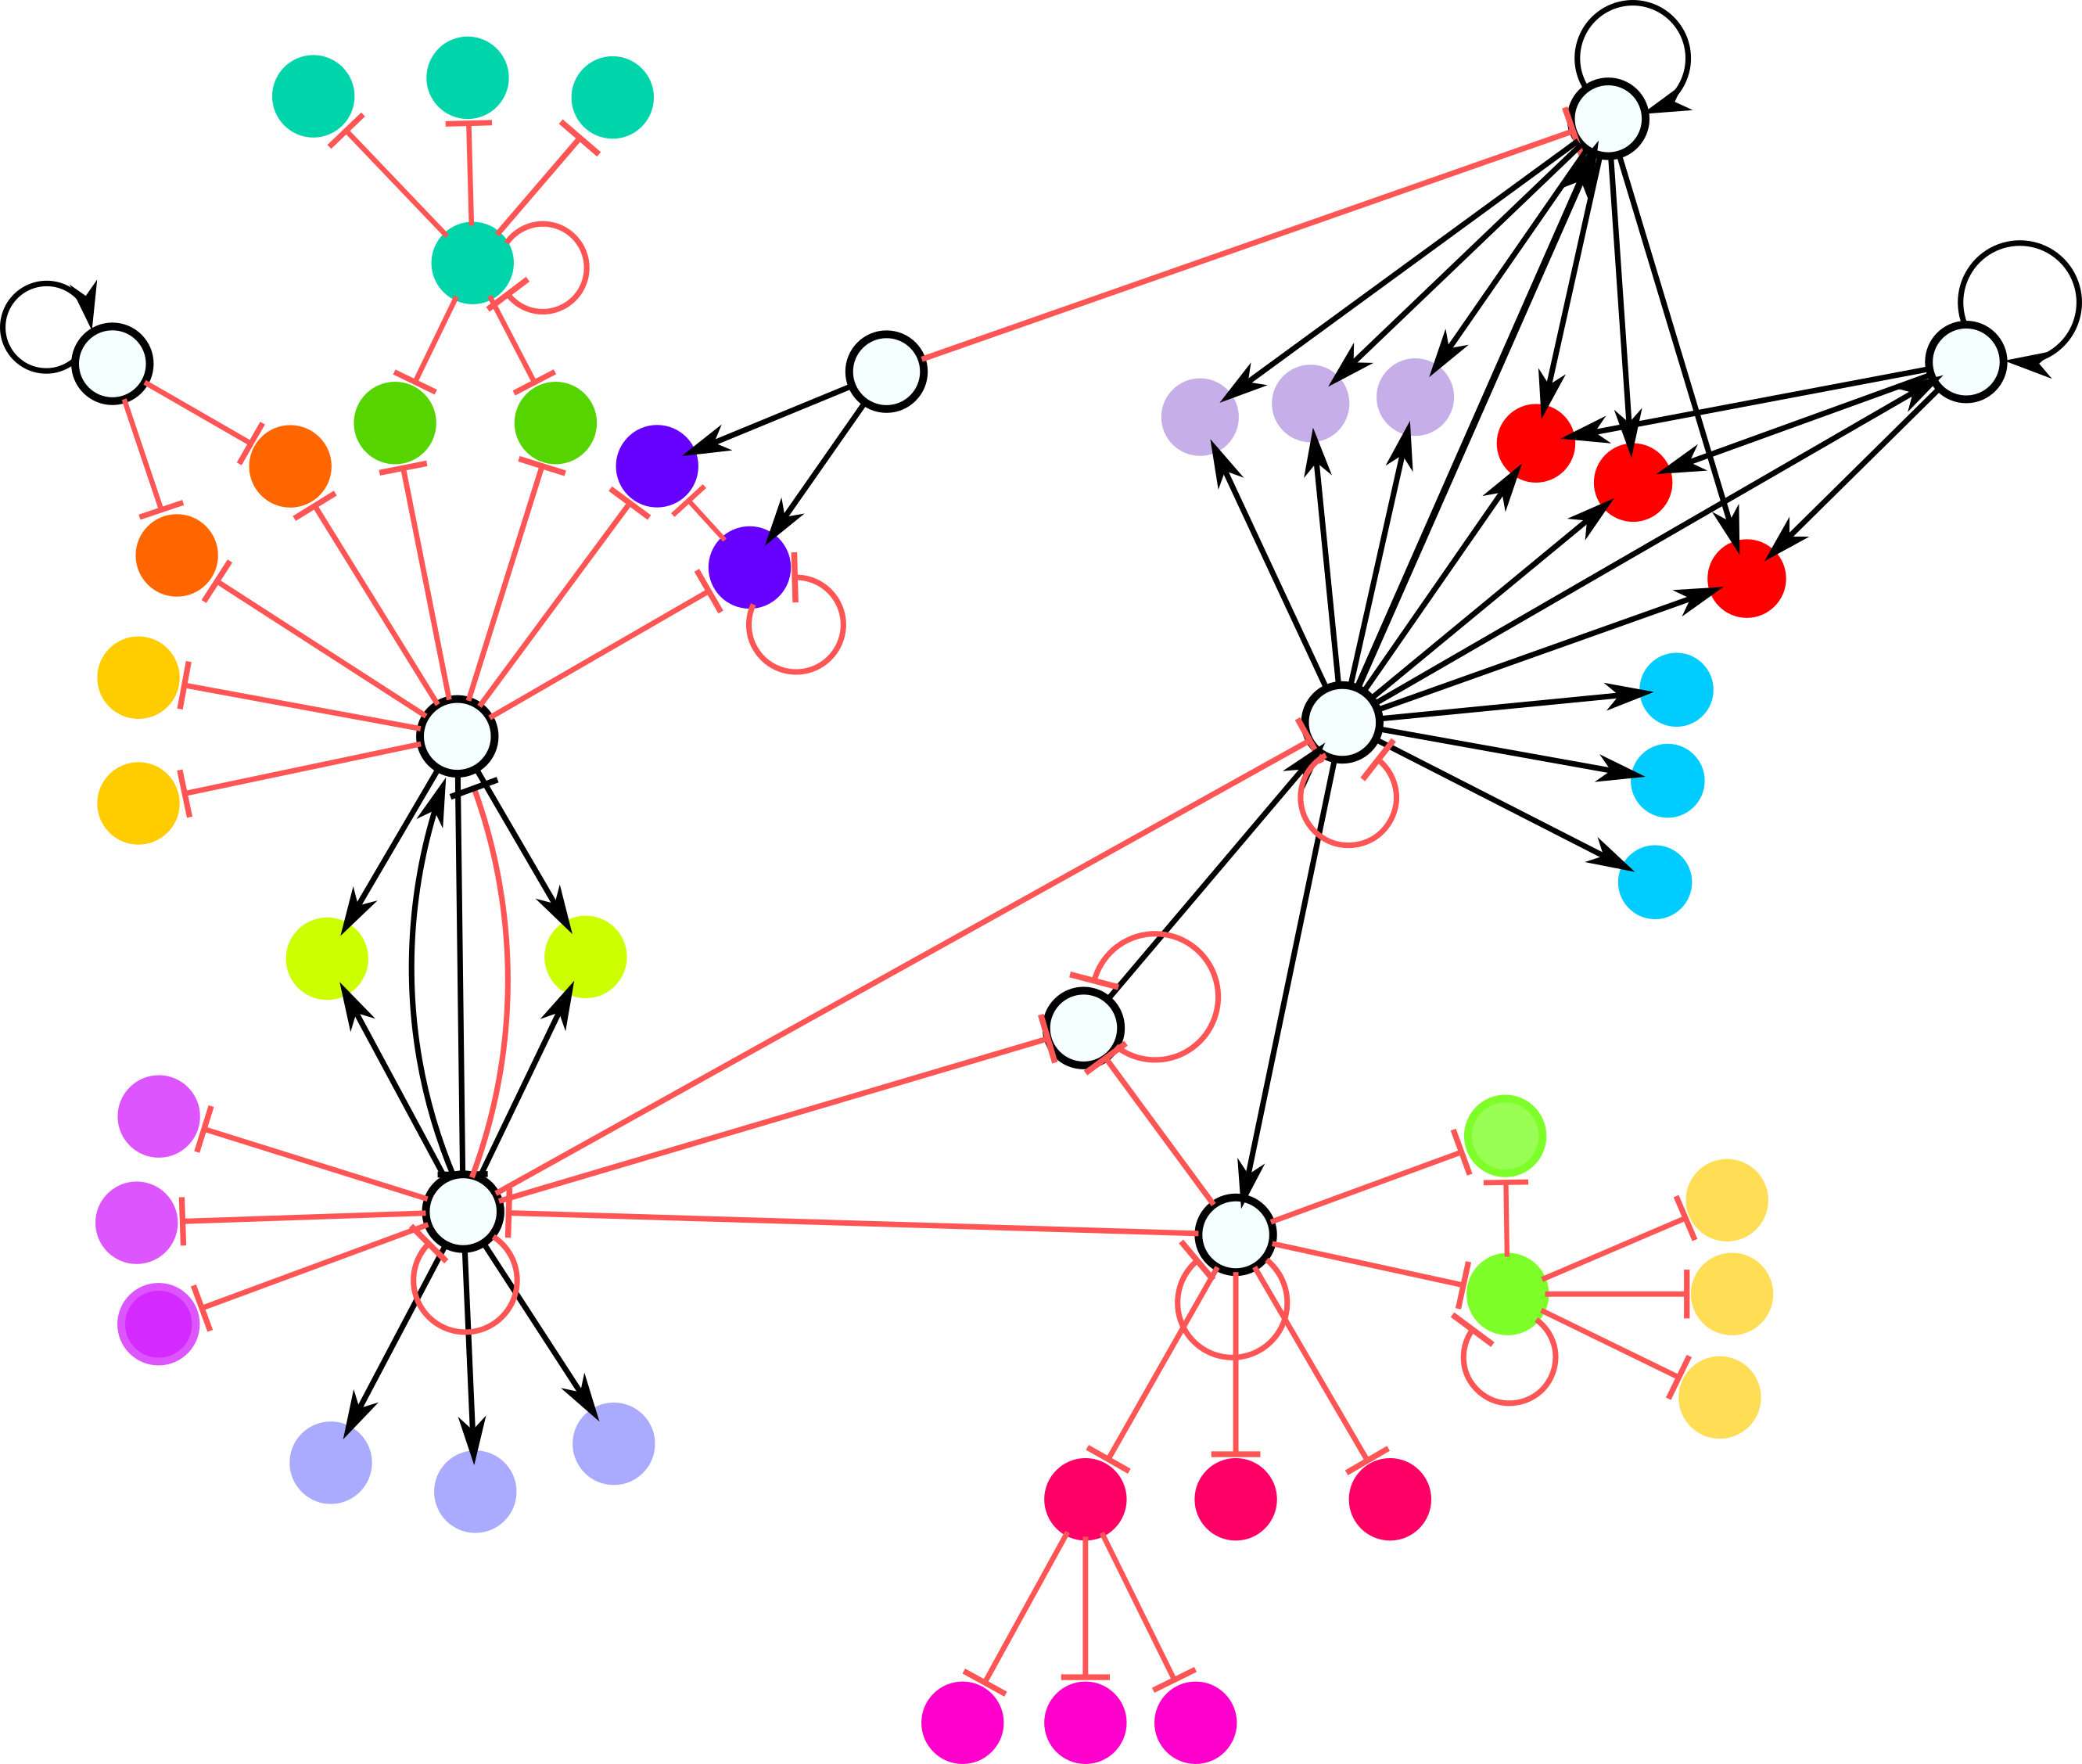
\includegraphics[scale=0.27]{Figures/result3-1.png}
	\caption{}
	\label{fig:result3-1}
\end{figure}

The connected component showed at the figure \ref{fig:result3} is a representation of a component in the whole regulatory network of the \textit{Escherichia Coli} bacteria and the resulted fibers shows just a portion of the whole fibers pattern. In the table X we give the classification for each fibration building block obtained for the whole bacteria network, including of course the fibers presented in the figure \ref{fig:result3-1}. In total, we have found $84$ non-trivial fiber groups containing a total of 462 nodes, obtaining a characteristic fiber statistics for the \textit{Escherichia Coli} network data. To guarantee the correctness of the fiber distribution found we calculate after the application of the refinement partitioning algorithm the information received for each node inside a fiber and compares if each one process equivalent information.

The statistics concerning the number of each fibration block on the network is given in the table X, showing \textcolor{red}{describe the pattern of the statistics of the table that concerns the bacteria fiber statistics}.


\section{Conclusion}

Nullam semper quam at ante convallis posuere. Ut faucibus tellus ac massa luctus consectetur. Nulla pellentesque tortor et aliquam vehicula. Maecenas imperdiet euismod enim ut pharetra. Suspendisse pulvinar sapien vitae placerat pellentesque. Nulla facilisi. Aenean vitae nunc venenatis, vehicula neque in, congue ligula.


%----------------------------------------------------------------------------------------
%	BIBLIOGRAPHY
%----------------------------------------------------------------------------------------

\bibliographystyle{unsrt}

\bibliography{sample.bib}

%----------------------------------------------------------------------------------------

\end{document}
